\begin{figure}%[h]
	\centering
	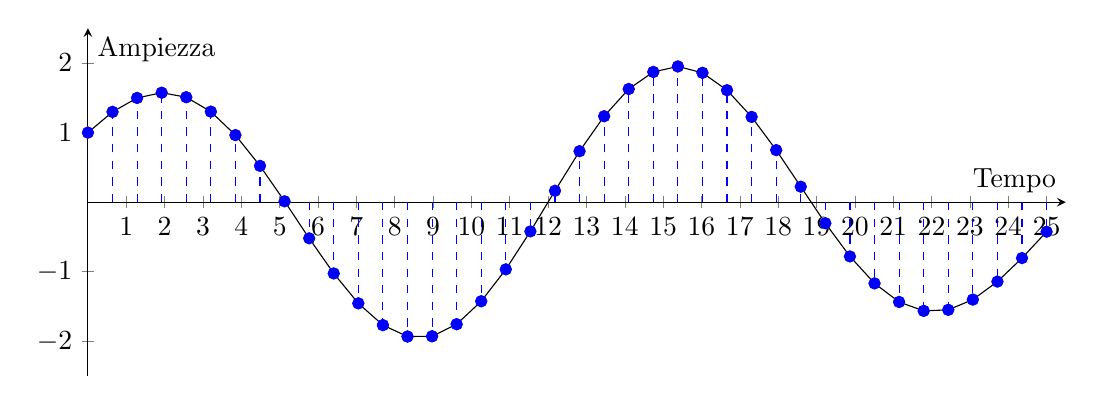
\begin{tikzpicture}[>=latex]
		\begin{axis}[
			axis lines = middle,
			xlabel = Tempo,
			ylabel = Ampiezza,
			xtick={0,1,...,25},
			ytick={-2,-1,...,2},
			xmin=0,
			xmax=25.5,
			ymin=-2.5,
			ymax=2.5,
			width=140mm,
			height=60mm,
			]
			\addplot[
			scatter,
			domain=0:25,
			samples=40,
			color=black
			]
			{sin(180*x/6)+cos(180*x/8)};
			\addplot[
			only marks,
			domain=0:25,
			samples=40,
			color=blue
			]{sin(180*x/6)+cos(180*x/8)};
			\addplot[
			ycomb,
			dashed,
			domain=0:25,
			samples=40,
			color=blue
			]
			{sin(180*x/6)+cos(180*x/8)};
		\end{axis}
	\end{tikzpicture}
	\caption{Campionamento di un segnale audio complesso. L'onda viene scomposta in campioni equidistanti che rappresentino l'ampiezza nel tempo, descrivendo l'onda originale.}
	\label{fig:campionamento}
\end{figure}